
\section{2D Solver}
The spatial domain for the 2D solver is $\Omega=[0\;\;1]\times[0\;\;1]$. To go about solving the system in 2D there are many options,
we compare two schemes: Lax-Wendfoff with dimenison splitting and a two step version by Richtmeyer. \newline

\subsection{Dimensional Splitting (Lax-Wendroff)}

Using the 1D equations of the Lax-Wendroff scheme for system (4) a dimenional split can be implemented by 
doing a step in $x$, followed by a step in $y$: 
\begin{equation}\label{eqn:6}
U_{ij}^* = U_{ij}^n - \frac{\Delta t}{2} 
\bigg(( I- \frac{\Delta t}{\Delta x} A_{i+\frac{1}{2}j}^n ) D_+^xF_{ij}^n 
+ (I+ \frac{\Delta t}{\Delta x} A_{i-\frac{1}{2}j}^n) D_{\_}^xF_{ij}^n\bigg)
\end{equation}
\begin{equation}\label{eqn:7}
U_{ij}^{n+1} = U_{ij}^* - 
\frac{\Delta t}{2} \bigg((I - \frac{\Delta t}{\Delta y} B_{ij+\frac{1}{2}}^*) D_+^yG_{ij}^*
 +(I + \frac{\Delta t}{\Delta x} B_{ij-\frac{1}{2}}^*) D_{\_}^y G_{ij}^* \bigg)
\end{equation}

As we see mixed derivatives will be treated non simmetricly by this formulas. We observe same oscilations as in 1D as in numerical solution.
Dimensional splitting turnes to be dramaticly unstable and to produce the numerical solution as on Figure~\ref{fig:2DSolutions_ds} timestep was decrised
2 times bellow the CFL condition and small ammout of artificial viscosity $0.03 \Delta x U_{xx}$ was added to a scheme. By the same argument as the initial condition
we chose smooth function (gaussian). 

\begin{figure}[h!]
    \centering
    \begin{subfigure}[t]{0.48\textwidth}
        \centering
        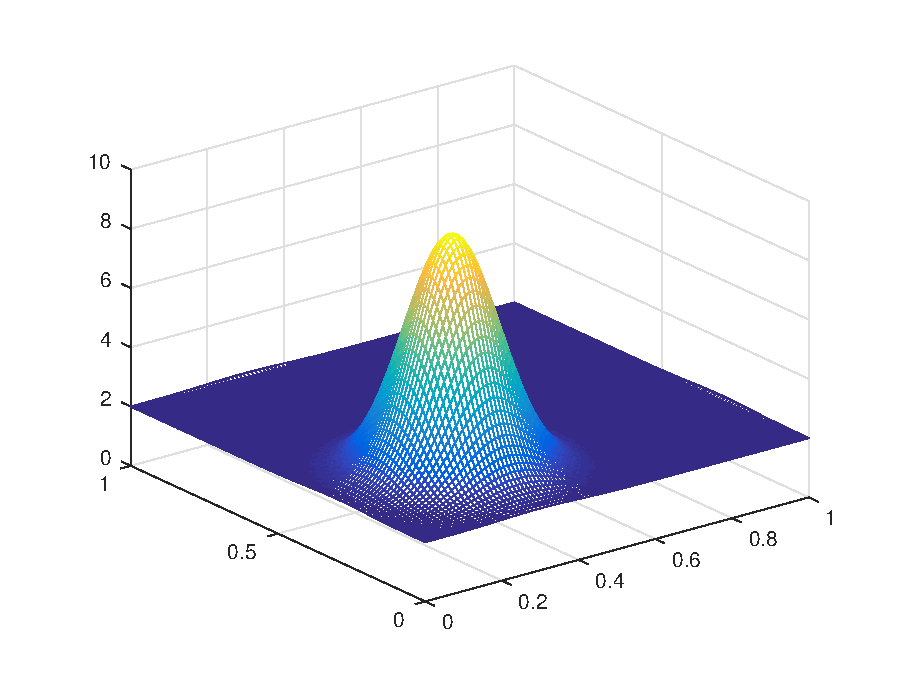
\includegraphics[width=\textwidth]{images/sol_ds_0000.eps}
        \caption{$n=0$}
        \label{fig:0}
    \end{subfigure}
    \begin{subfigure}[t]{0.48\textwidth}
        \centering
        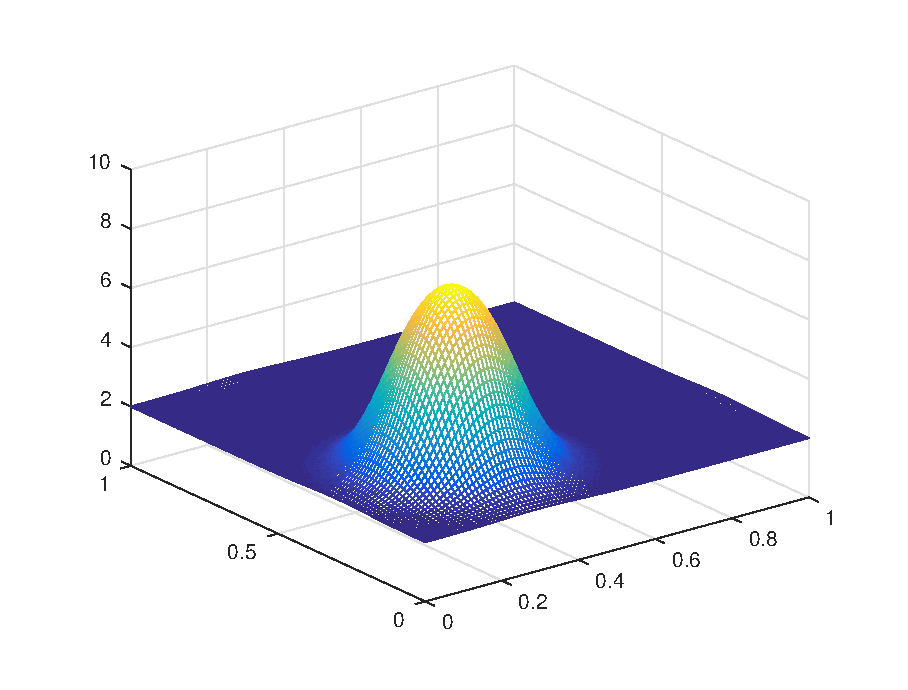
\includegraphics[width=\textwidth]{images/sol_ds_0010.eps}
        \caption{$n=10$}
        \label{fig:10}
    \end{subfigure}
    \begin{subfigure}[t]{0.48\textwidth}
        \centering
        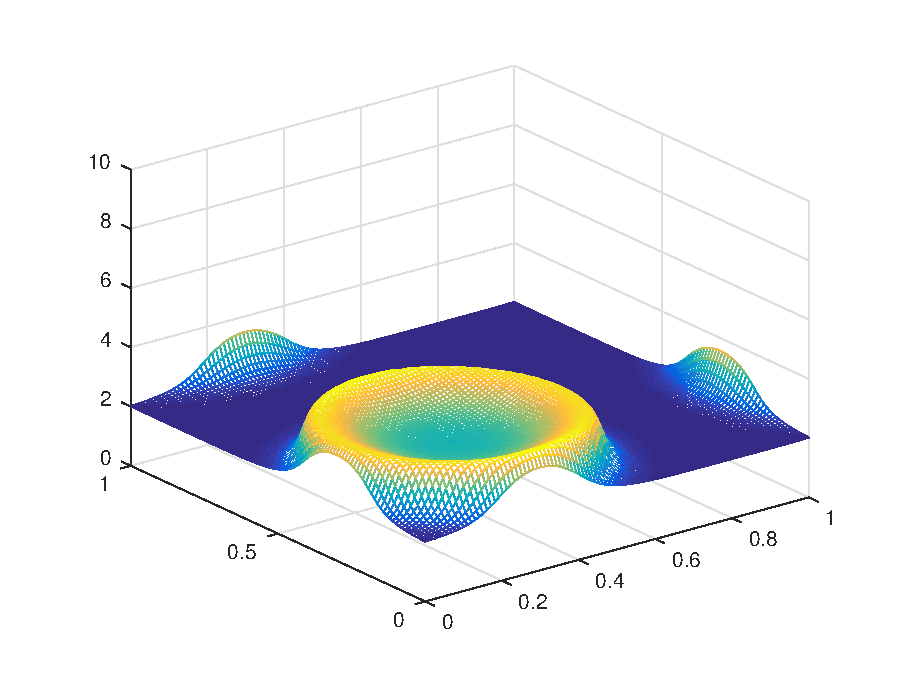
\includegraphics[width=\textwidth]{images/sol_ds_0050.eps}
        \caption{$n=50$}
        \label{fig:50}
    \end{subfigure}
    \begin{subfigure}[t]{0.48\textwidth}
        \centering
        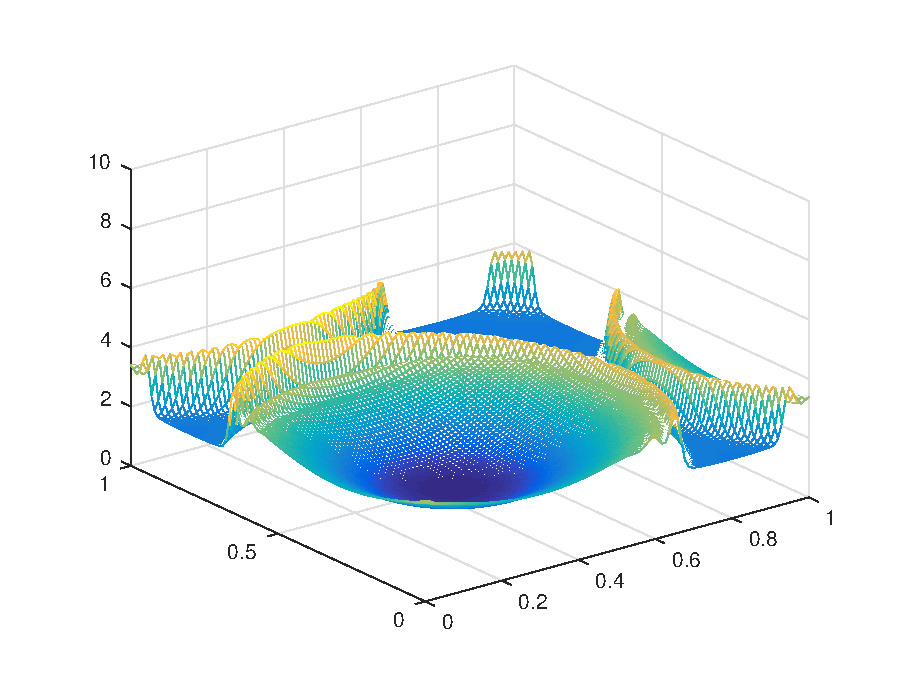
\includegraphics[width=\textwidth]{images/sol_ds_0100.eps}
        \caption{$n=100$}
        \label{fig:100}
    \end{subfigure}
    \caption{Periodic boundary condtions for dimensional splitting.}
    \label{fig:2DSolutions_ds}
\end{figure}

\begin{figure}[h!]
    \centering
    \begin{subfigure}[t]{0.4\textwidth}
        \centering
        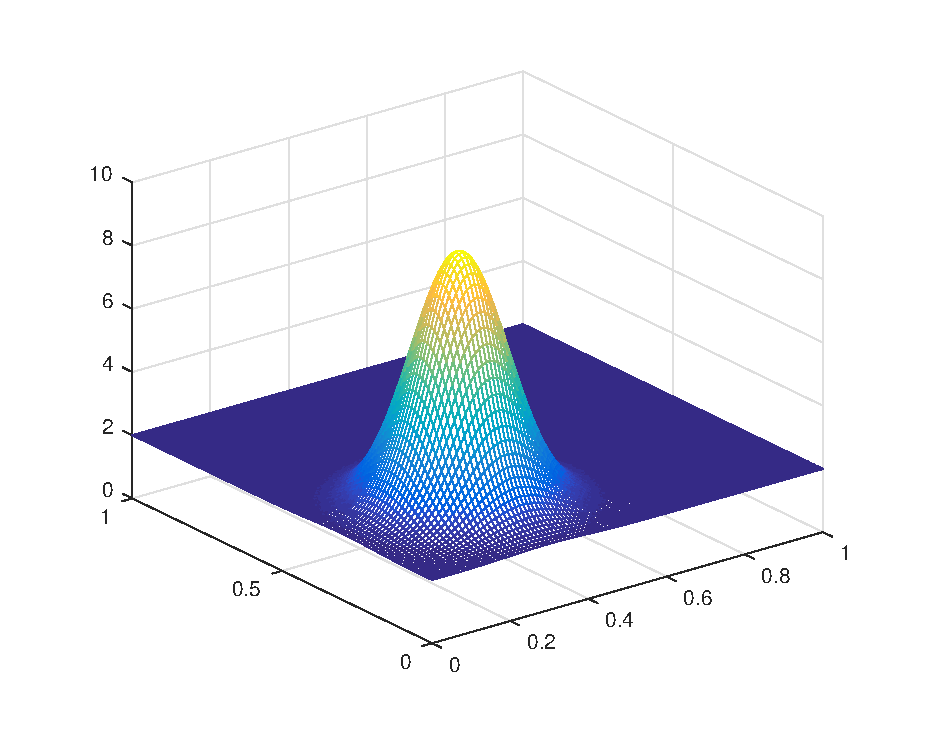
\includegraphics[width=\textwidth]{images/sol_ds_0000_per.eps}
        \caption{$n=0$}
        \label{fig:0}
    \end{subfigure}
    \begin{subfigure}[t]{0.48\textwidth}
        \centering
        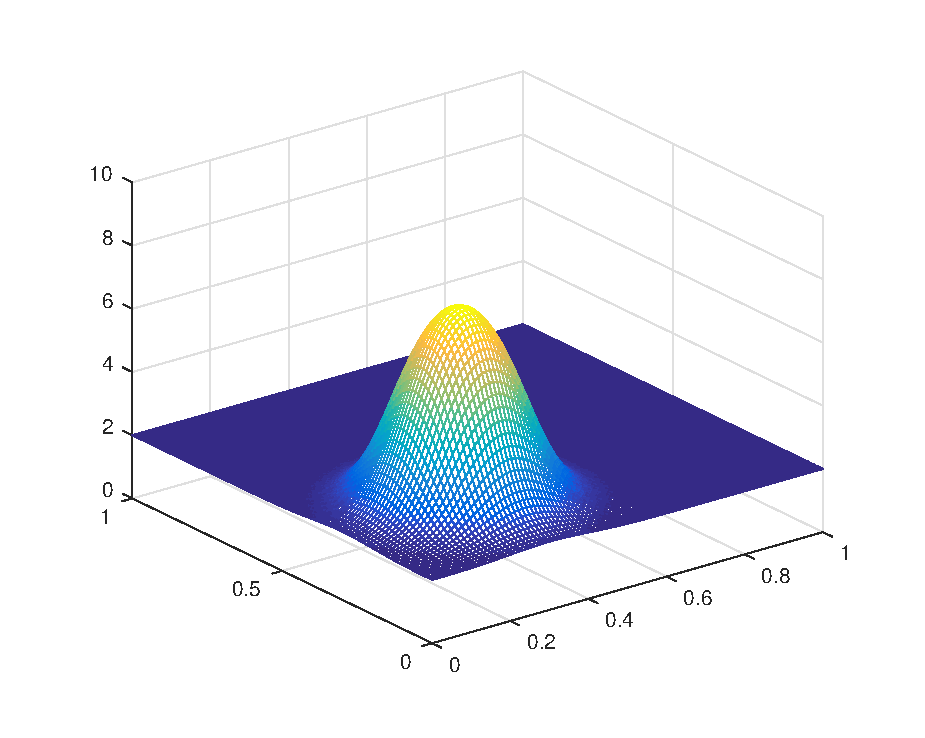
\includegraphics[width=\textwidth]{images/sol_ds_0010_per.eps}
        \caption{$n=10$}
        \label{fig:10}
    \end{subfigure}
    \begin{subfigure}[t]{0.48\textwidth}
        \centering
        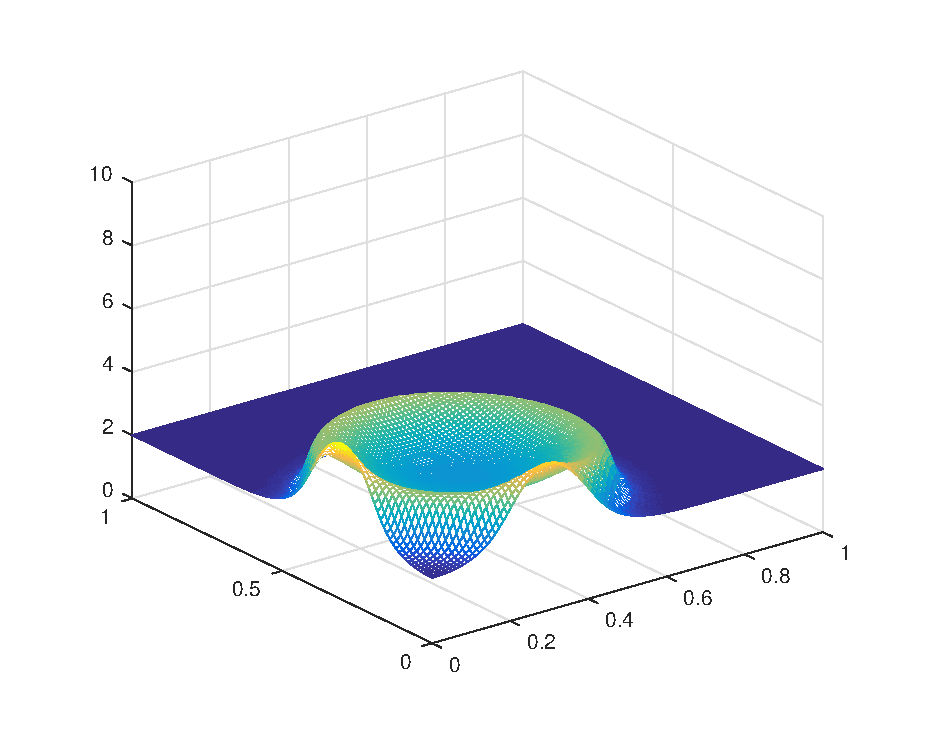
\includegraphics[width=\textwidth]{images/sol_ds_005_per.eps}
        \caption{$n=50$}
        \label{fig:50}
    \end{subfigure}
    \begin{subfigure}[t]{0.48\textwidth}
        \centering
        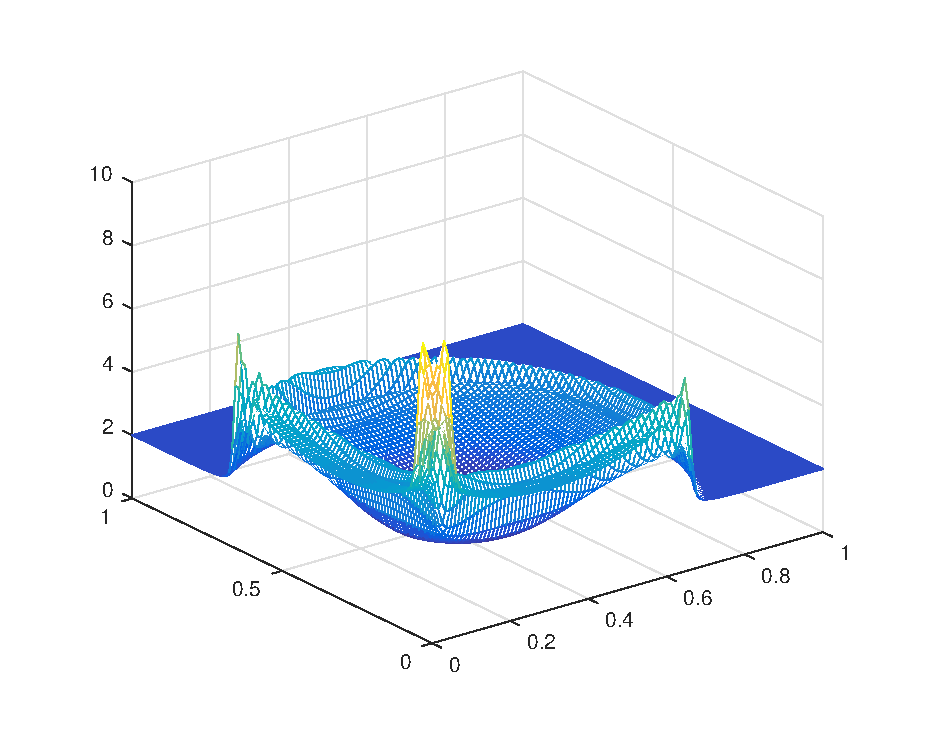
\includegraphics[width=\textwidth]{images/sol_ds_0100_per.eps}
        \caption{$n=100$}
        \label{fig:100}
    \end{subfigure}
    \caption{Free boundary condtions for dimensional splitting.}
    \label{fig:2DSolutions_ds}
\end{figure}

\subsection{Two-Step Lax-Wendroff Method (Richtmeyer)}

Richtmeyer proposed a two-step version of the Lax-Wendroff method \cite{Roach}, which is much simpler than the original, especially in multi-dimensional problems.
The first step uses Lax's method and the second step is a midpoint leapfrog calculation. 

\begin{equation}\label{eqn:8}
U_{i}^{n+1} = \frac{1}{2}(U_{i+1}^{n}+U_{i-1}^{n})-\Delta{t} \Big(\frac{F_{i+1}^{n}-F_{i-1}^{n}}{2\Delta x}\Big)
\end{equation}
\begin{equation}\label{eqn:9}
U_{i}^{n+2} = U_{i}^{n+1} + (2\Delta t) \Big ( \frac{ F_{i+1}^{n+1}-F_{i-1}^{n+1} }{ 2 \Delta x } \Big)
\end{equation} 
\newline

The values $F_{i \pm 1}^{n+1}$ in the second step are based on the $U_{i \pm 1}^{n+1}$ results of the first step. The first step is considered
a provisonal step, with signifigance attached only to the results of the second step in each sequence. This method does not look anything like the original
Lax-Wendroff method of \eqref{eqn:4}, but substitution of \eqref{eqn:10} and \eqref{eqn:11} shows that the methods are equivalent. 
\newline
The extension to multiple dimensions is obvious and neat.
\begin{equation}\label{eqn:10}
\frac{\partial U}{\partial t} = - \Big( \frac{\partial F}{\partial x} + \frac{\partial G}{\partial y} \Big)
\end{equation}

\begin{dmath}\label{eqn:11}
U_{ij}^{n+1} = \frac{1}{4} \Big( U_{i+1,j}^{n} + U_{i-1,j}^{n} + U_{ij+1}^{n} + U_{ij-1}^{n} \Big) 
- (\Delta t) \Big( \frac{ F_{i+1,j}^{n} - F_{i-1,j}^{n} }{2 \Delta x}  + \frac{ G_{ij+1}^{n} - G_{ij-1}^{n} }{ 2 \Delta y }  \Big)
\end{dmath}
\begin{dmath}\label{eqn:11_1}
U_{ij}^{n+2} = U_{i,j}^{n+1} -
  (2\Delta t) \Big( \frac{ F_{i+1,j}^{n+1} - F_{i-1,j}^{n+1} }{2 \Delta x}  + \frac{ G_{ij+1}^{n+1} - G_{ij-1}^{n+1} }{ 2 \Delta y }  \Big)
\end{dmath} 

This 2D-scheme requires about a fourth of the computational time as the original Lax-Wendroff method, and produces less shock
overshoot than the orignal\cite{Roach}. It is worth it to note that the Ricthmeyer scheme does not require evalutaion
of the Jacobians. 
\newline

The boundary conditions are prescribed for two cases. The first, periodic for both $h$, $hu$, and $hv$, and the second,
and more complicated conditions, free for $h$, reflective in the horizontal direction and free in the vertical direction 
for $uh$, and reflective in the vertical direction and free in the horizontal direction for $vh$. 
The initial conditions are then chosen to be piecewise, 

\begin{equation}\label{eqn:12}
u_0(x,y)=
\begin{array}{ll}
\Big\{ & 
\begin{array}{ll}
 8, & \text{if} (x-0.3)^2+(y-0.3)^2 \\
 1, & \text{otherwise} \\
\end{array}
\end{array}
\end{equation}

interestingly forming a cylindrical column. Note that Dimenional splitting could not treat discontinous initial conditions while Richtmeyer scheme remained stable
without any artificial viscosity. The Corilis force was added to  simulation with interesting boundary conditions (free for $h$, free for $hu$ in horizontal direction and reflective in vertical,
free for $hv$ in vertical direction and reflective in horizontal direction. 
\begin{figure}[h!]
    \centering
    \begin{subfigure}[t]{0.4\textwidth}
        \centering
        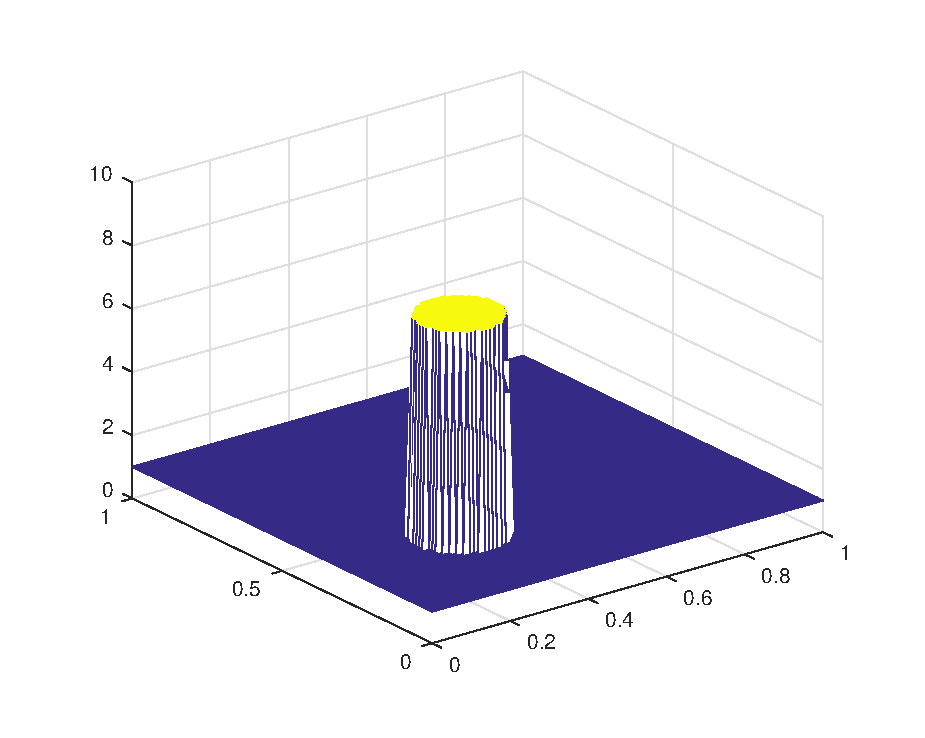
\includegraphics[width=\textwidth]{images/sol_ri_0000_per.eps}
        \caption{$n=0$}
        \label{fig:0}
    \end{subfigure}
    \begin{subfigure}[t]{0.48\textwidth}
        \centering
        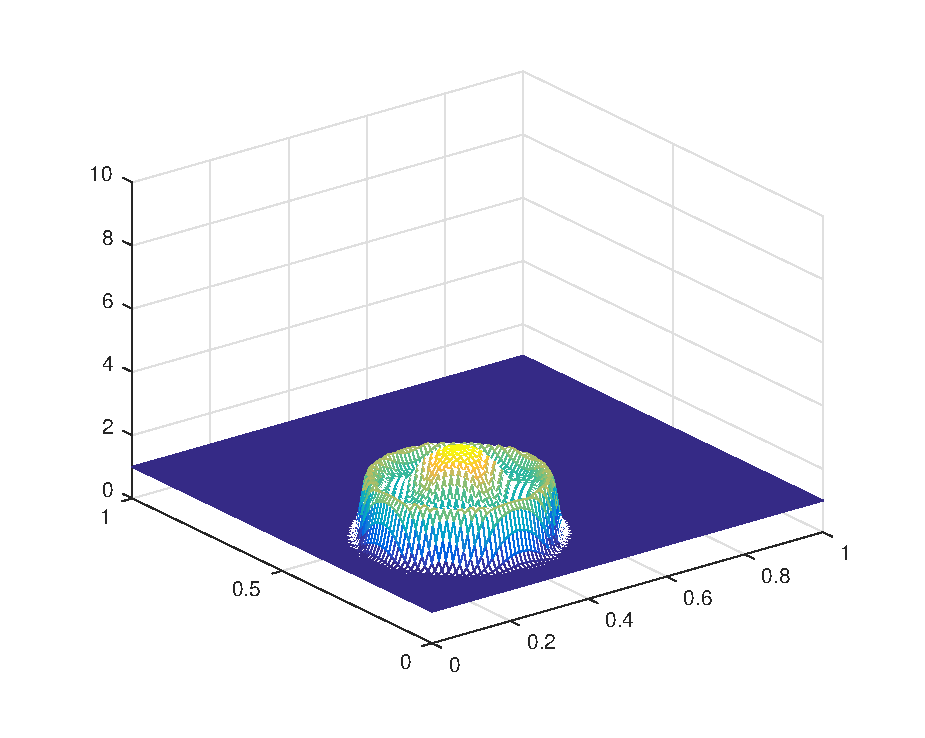
\includegraphics[width=\textwidth]{images/sol_ri_0025_per.eps}
        \caption{$n=25$}
        \label{fig:10}
    \end{subfigure}
    \begin{subfigure}[t]{0.48\textwidth}
        \centering
        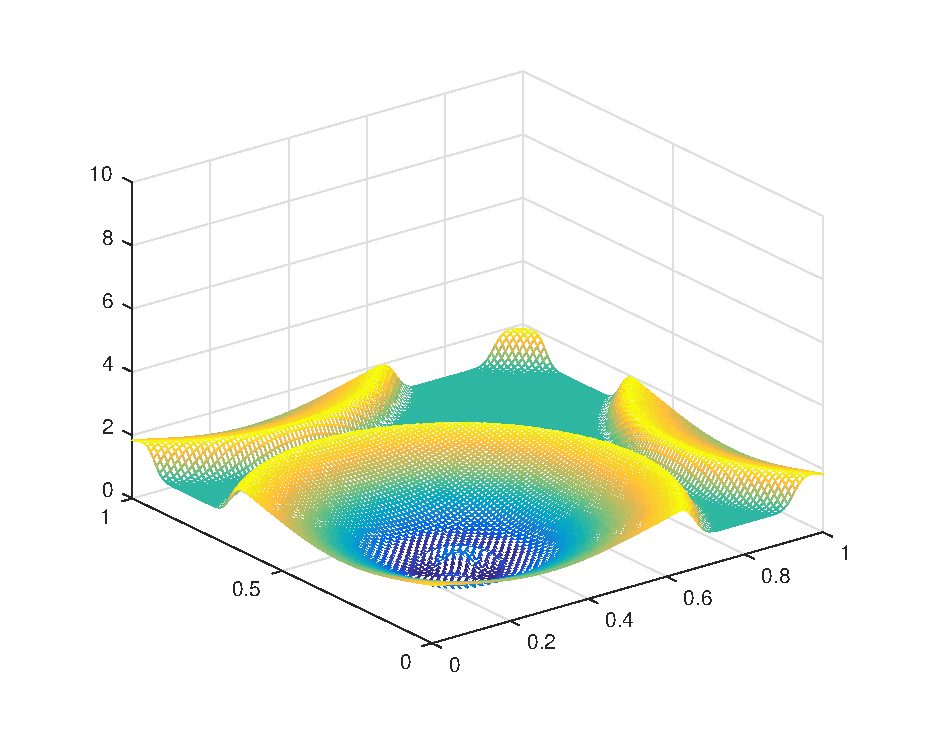
\includegraphics[width=\textwidth]{images/sol_ri_0100_per.eps}
        \caption{$n=100$}
        \label{fig:50}
    \end{subfigure}
    \begin{subfigure}[t]{0.48\textwidth}
        \centering
        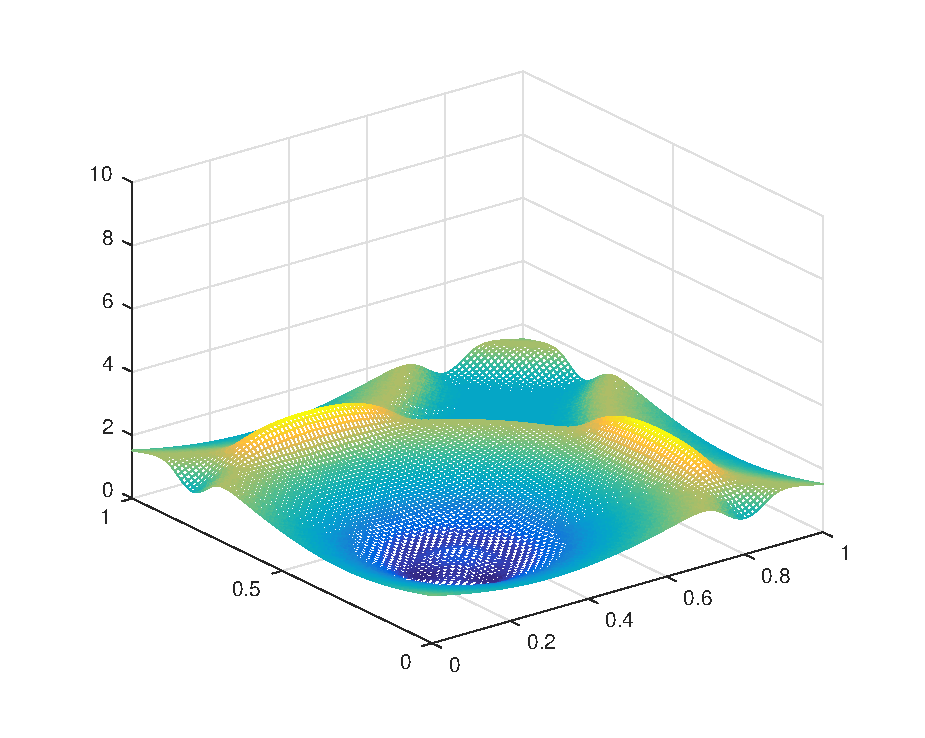
\includegraphics[width=\textwidth]{images/sol_ri_0150_per.eps}
        \caption{$n=150$}
        \label{fig:100}
    \end{subfigure}
    \begin{subfigure}[t]{0.48\textwidth}
        \centering
        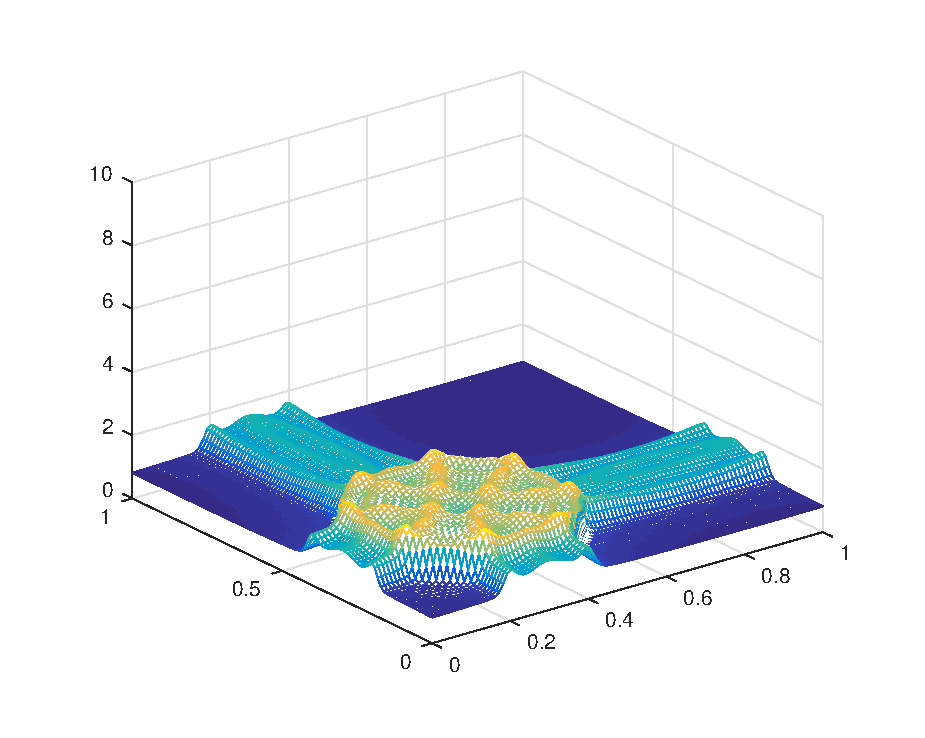
\includegraphics[width=\textwidth]{images/sol_ri_0400_per.eps}
        \caption{$n=400$}
        \label{fig:100}
    \end{subfigure}
    \begin{subfigure}[t]{0.48\textwidth}
        \centering
        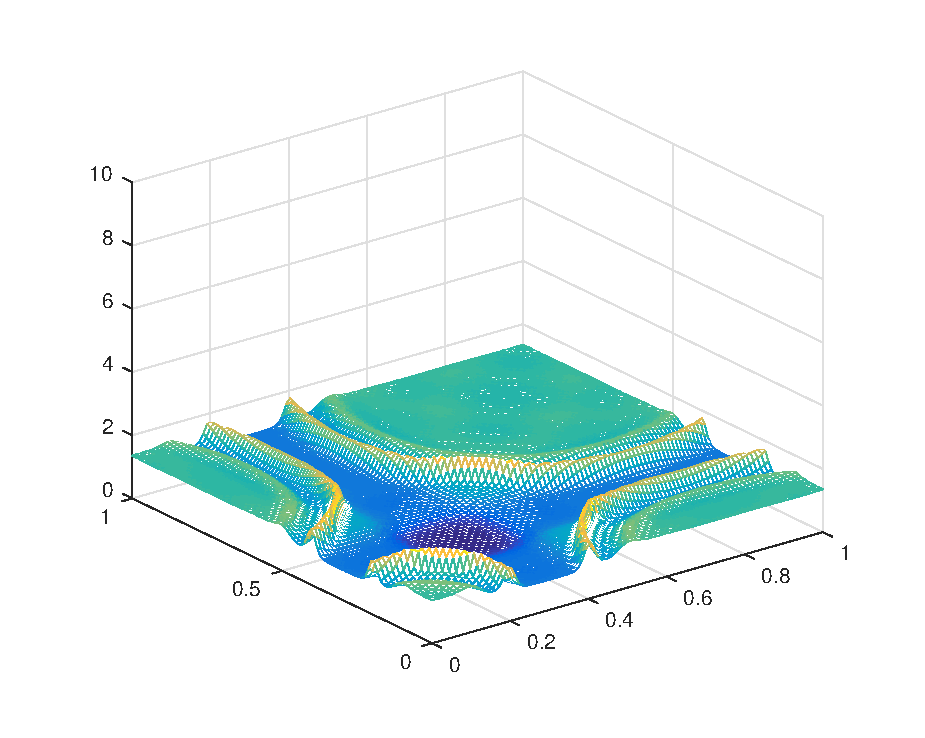
\includegraphics[width=\textwidth]{images/sol_ri_0600_per.eps}
        \caption{$n=600$}
        \label{fig:100}
    \end{subfigure}
    \begin{subfigure}[t]{0.48\textwidth}
        \centering
        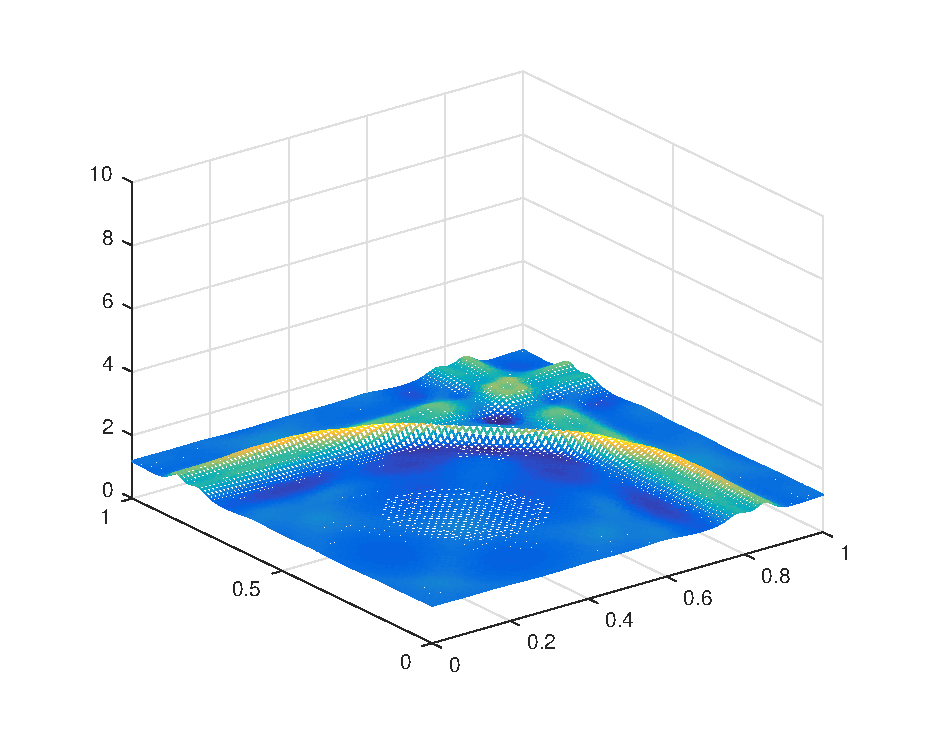
\includegraphics[width=\textwidth]{images/sol_ri_1000_per.eps}
        \caption{$n=1000$}
        \label{fig:100}
    \end{subfigure}
    \caption{Periodic boundary condtions for Richtmeyer scheme.}
    \label{fig:2DSolutions_ri}
\end{figure}
\begin{figure}[h!]
    \centering
    \begin{subfigure}[t]{0.4\textwidth}
        \centering
        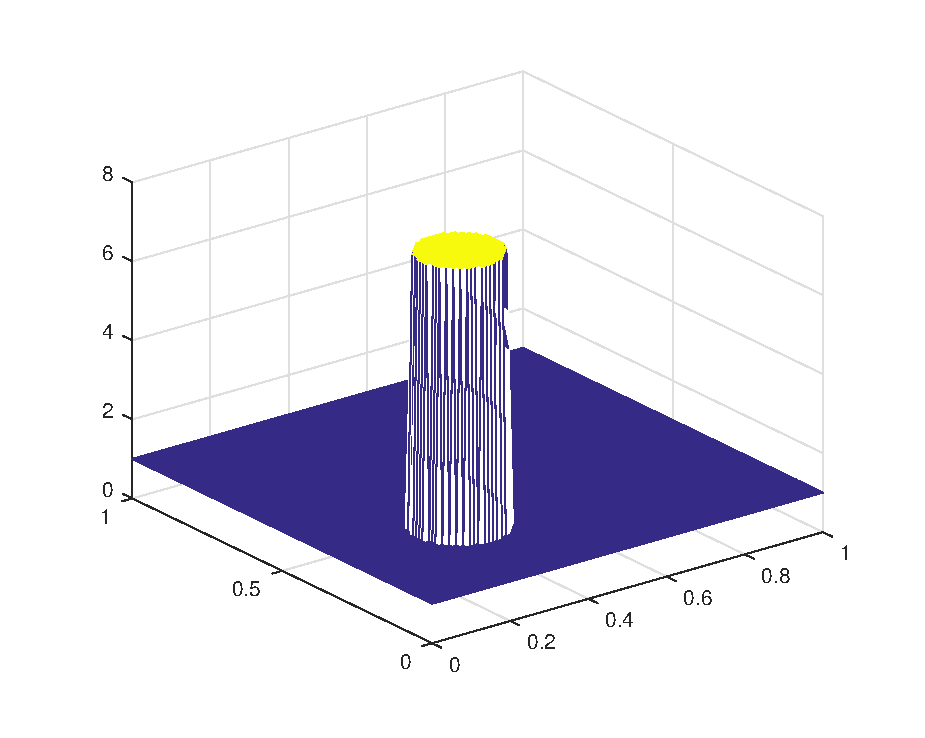
\includegraphics[width=\textwidth]{images/sol_ri_0000.eps}
        \caption{$n=0$}
        \label{fig:0}
    \end{subfigure}
    \begin{subfigure}[t]{0.48\textwidth}
        \centering
        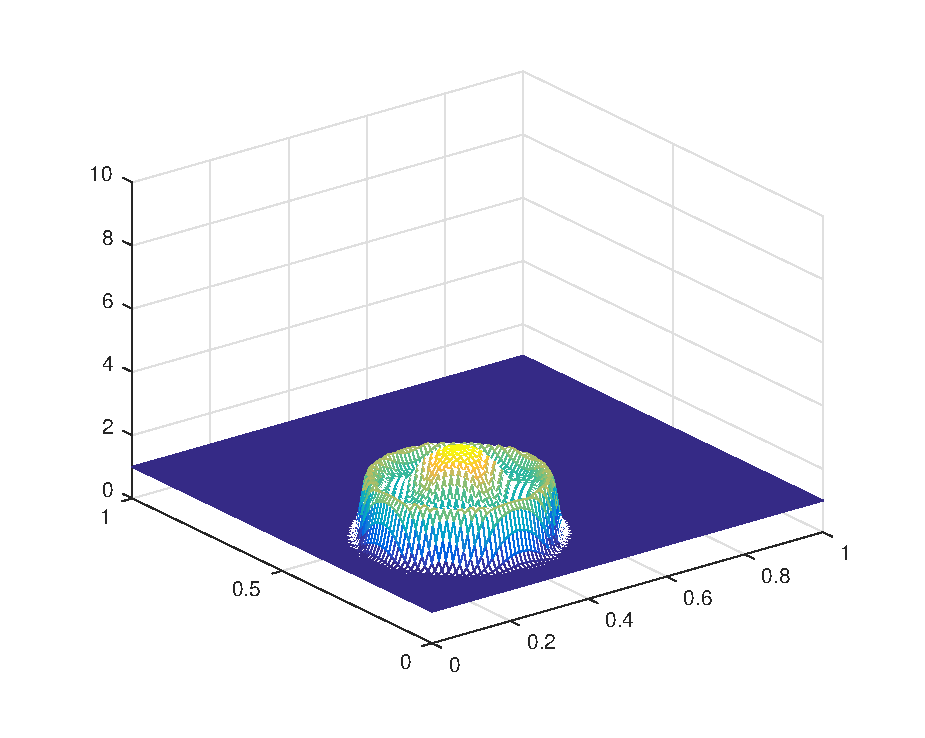
\includegraphics[width=\textwidth]{images/sol_ri_0025.eps}
        \caption{$n=25$}
        \label{fig:10}
    \end{subfigure}
    \begin{subfigure}[t]{0.48\textwidth}
        \centering
        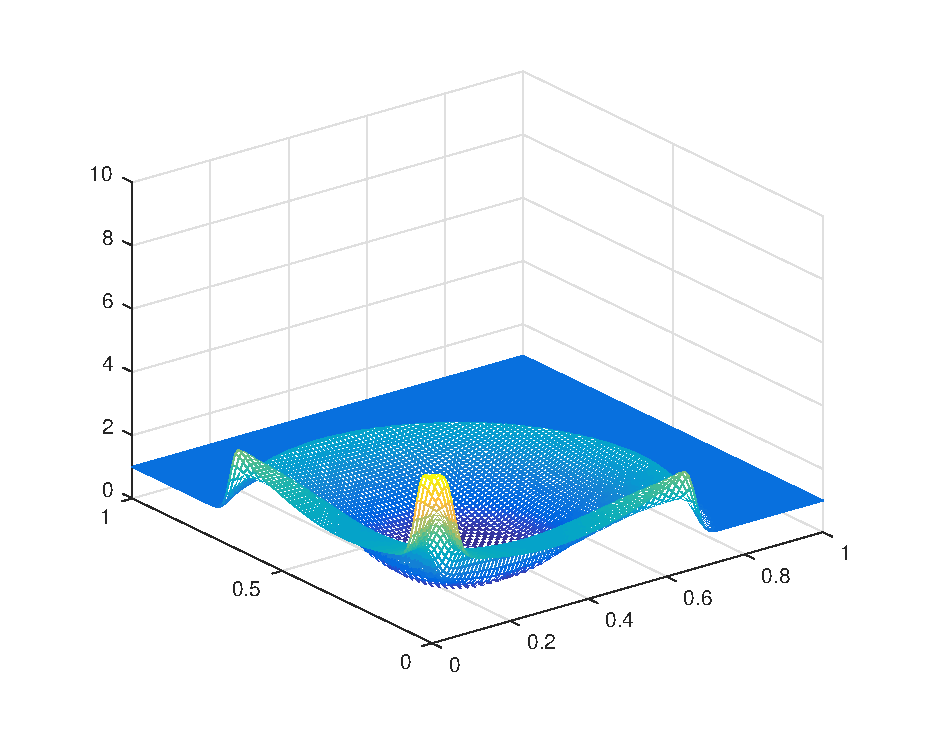
\includegraphics[width=\textwidth]{images/sol_ri_0100.eps}
        \caption{$n=100$}
        \label{fig:50}
    \end{subfigure}
    \begin{subfigure}[t]{0.48\textwidth}
        \centering
        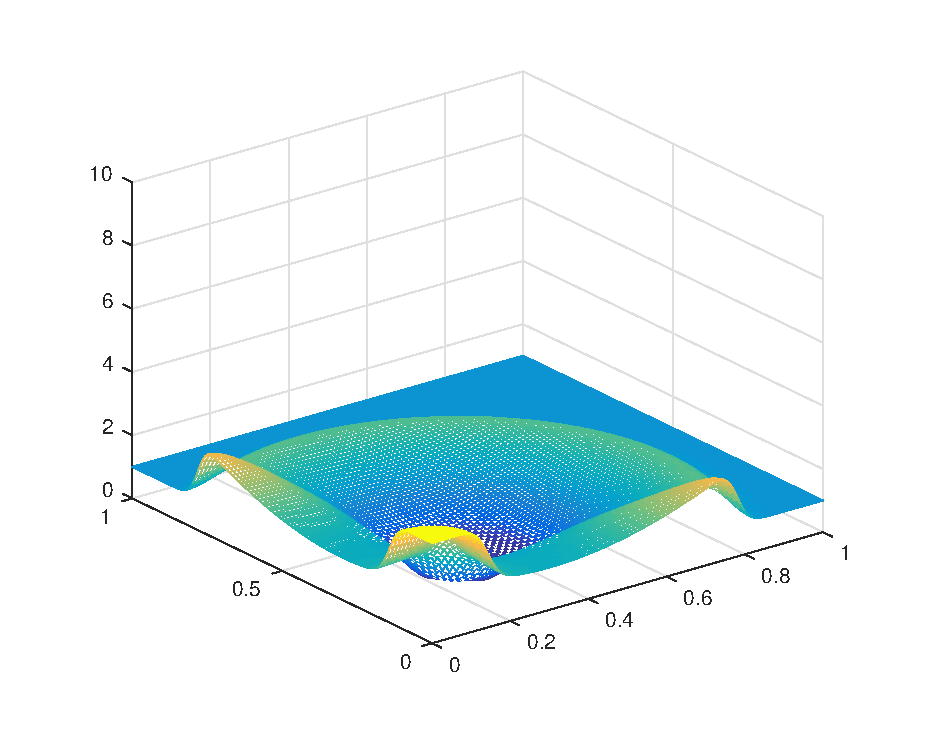
\includegraphics[width=\textwidth]{images/sol_ri_0150.eps}
        \caption{$n=150$}
        \label{fig:100}
    \end{subfigure}
    \begin{subfigure}[t]{0.48\textwidth}
        \centering
        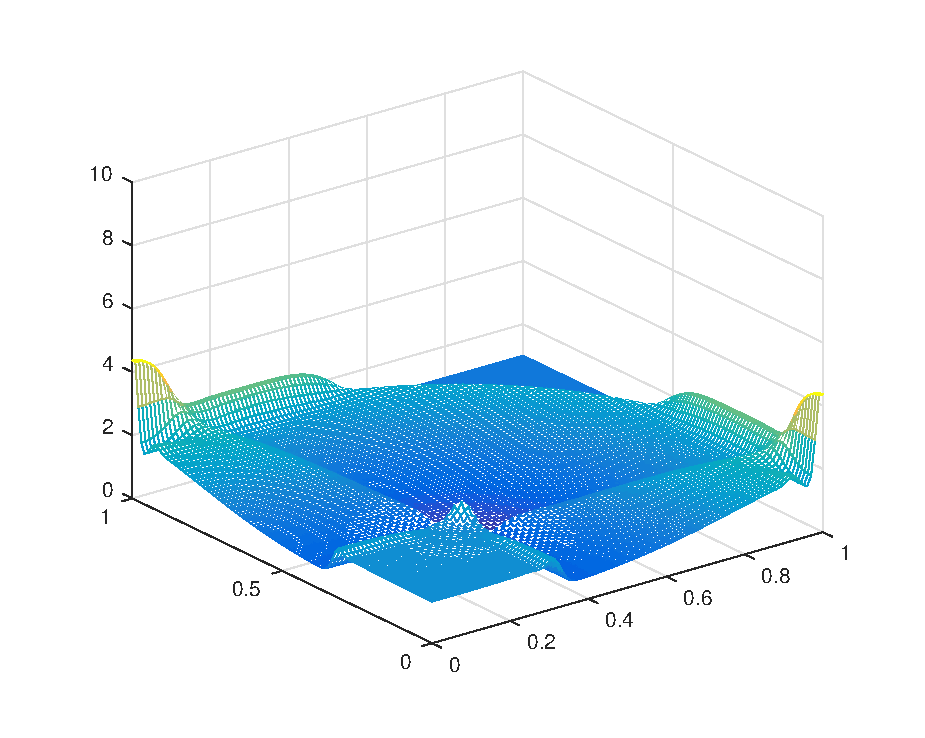
\includegraphics[width=\textwidth]{images/sol_ri_0400.eps}
        \caption{$n=400$}
        \label{fig:100}
    \end{subfigure}
    \begin{subfigure}[t]{0.48\textwidth}
        \centering
        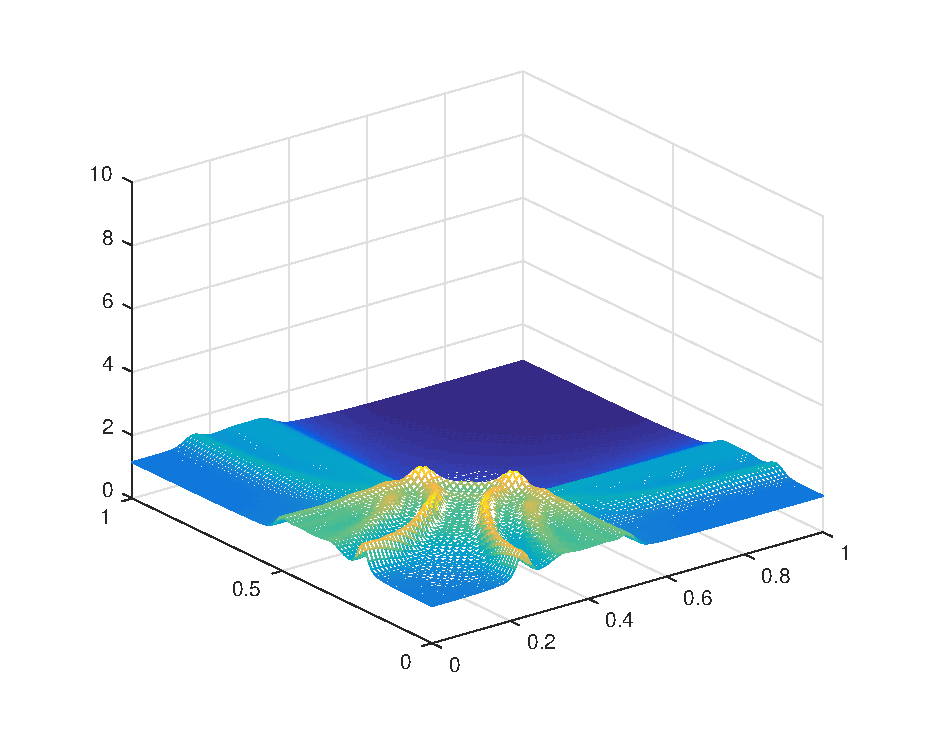
\includegraphics[width=\textwidth]{images/sol_ri_0600.eps}
        \caption{$n=600$}
        \label{fig:100}
    \end{subfigure}
    \begin{subfigure}[t]{0.48\textwidth}
        \centering
        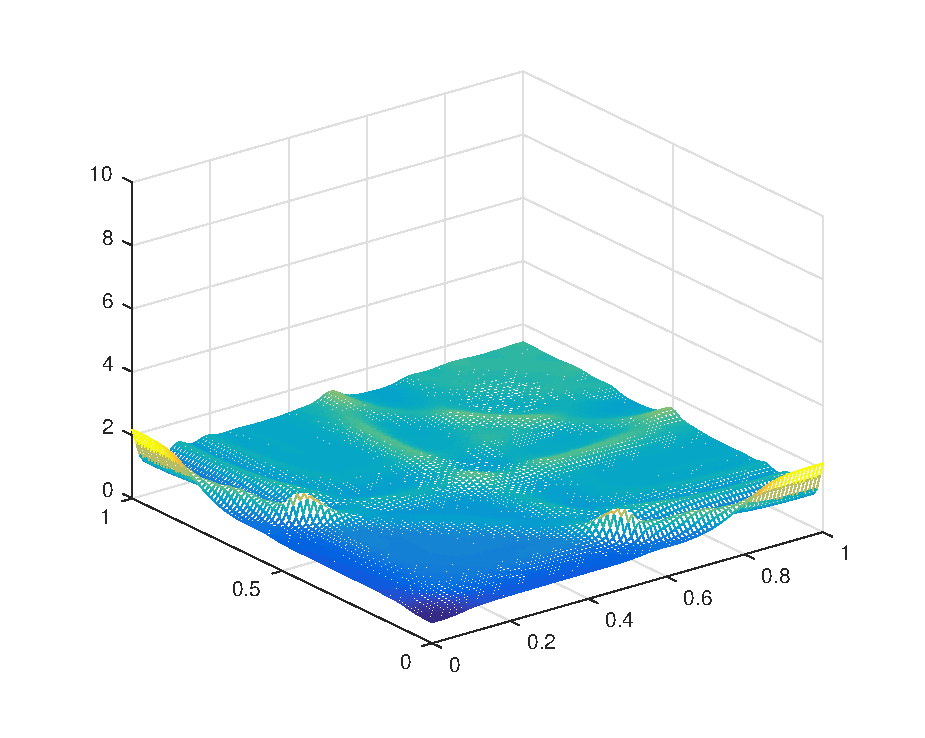
\includegraphics[width=\textwidth]{images/sol_ri_1000.eps}
        \caption{$n=1000$}
        \label{fig:100}
    \end{subfigure}
    \caption{Free boundary condtions for Richtmeyer scheme.}
    \label{fig:2DSolutions_ri}
\end{figure}

\begin{figure}[h!]
    \centering
    \begin{subfigure}[t]{0.4\textwidth}
        \centering
        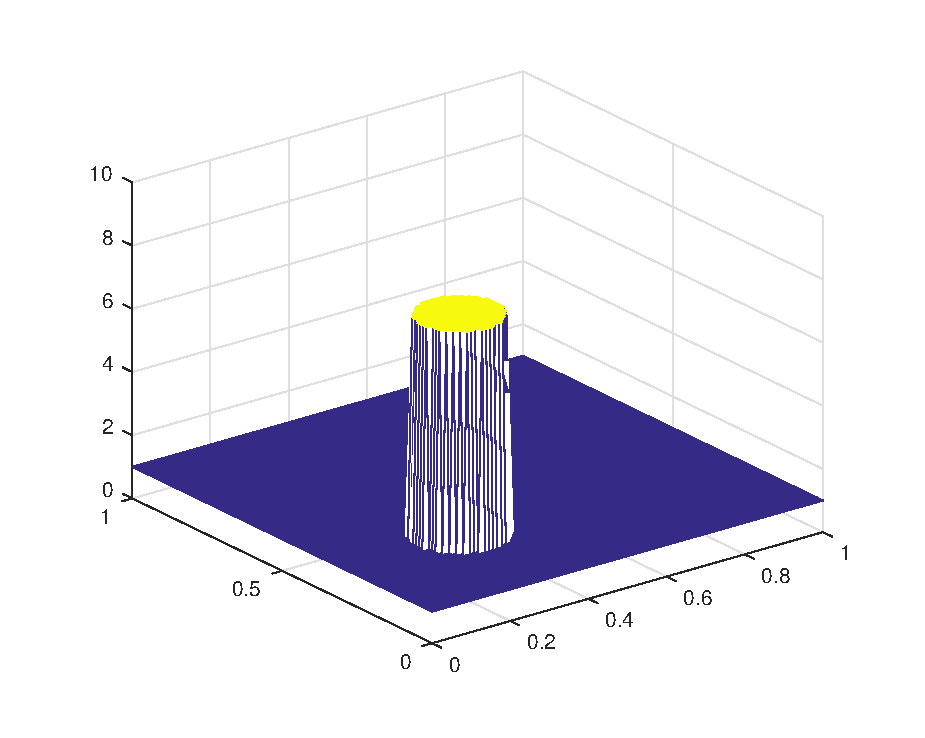
\includegraphics[width=\textwidth]{images/sol_ri_0000cf.eps}
        \caption{$n=0$}
        \label{fig:0}
    \end{subfigure}
    \begin{subfigure}[t]{0.48\textwidth}
        \centering
        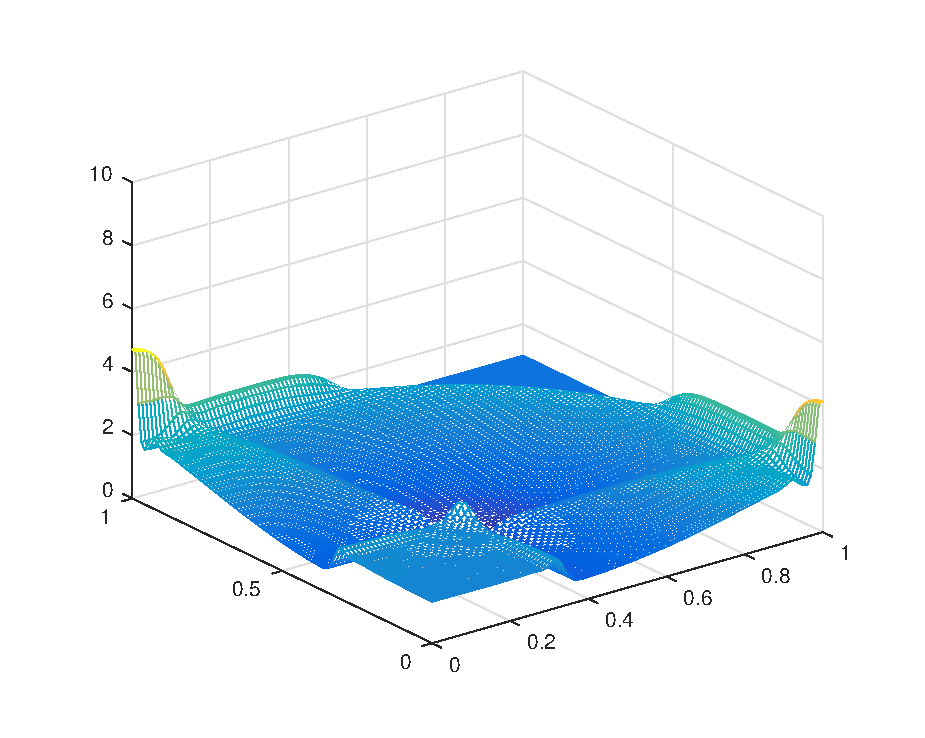
\includegraphics[width=\textwidth]{images/sol_ri_0200cf.eps}
        \caption{$n=200$}
        \label{fig:10}
    \end{subfigure}
    \begin{subfigure}[t]{0.48\textwidth}
        \centering
        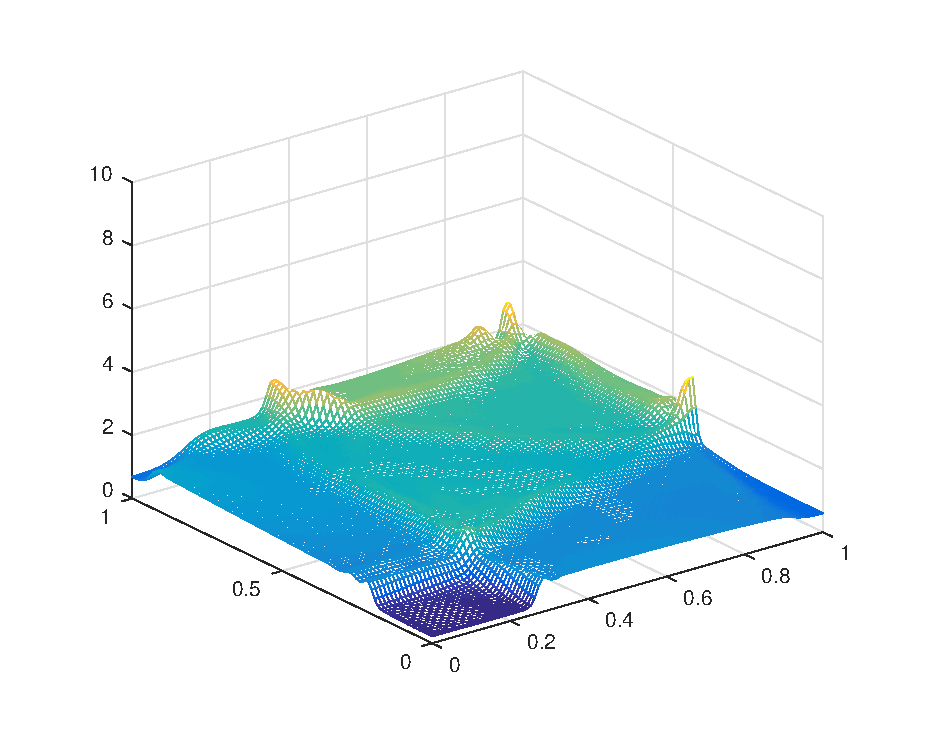
\includegraphics[width=\textwidth]{images/sol_ri_0400cf.eps}
        \caption{$n=400$}
        \label{fig:50}
    \end{subfigure}
    \begin{subfigure}[t]{0.48\textwidth}
        \centering
        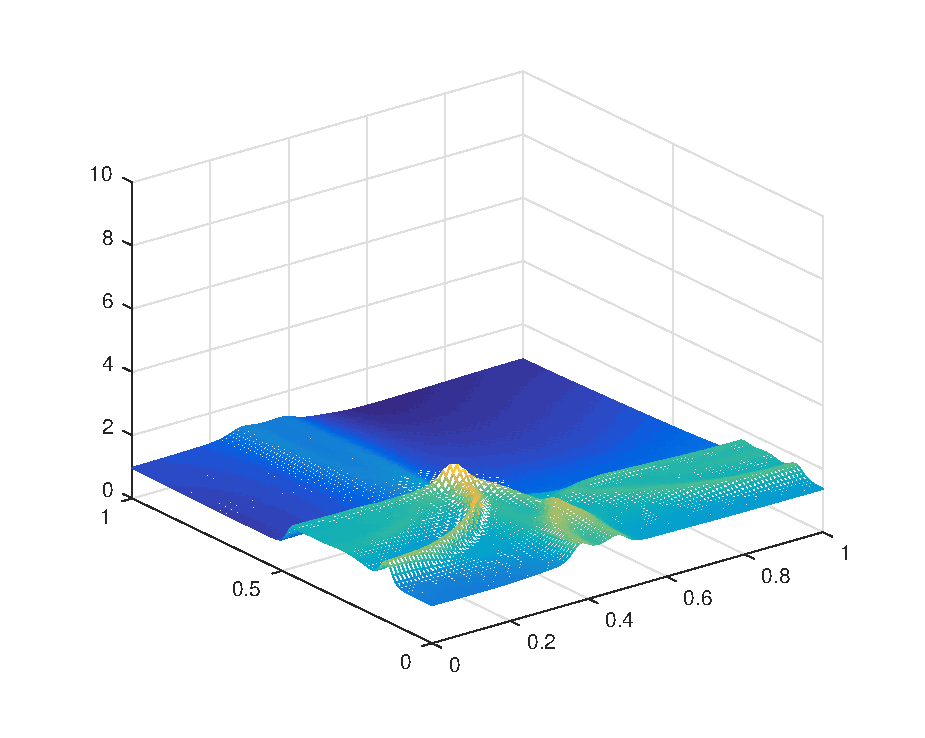
\includegraphics[width=\textwidth]{images/sol_ri_0600cf.eps}
        \caption{$n=600$}
        \label{fig:100}
    \end{subfigure}
    \begin{subfigure}[t]{0.48\textwidth}
        \centering
        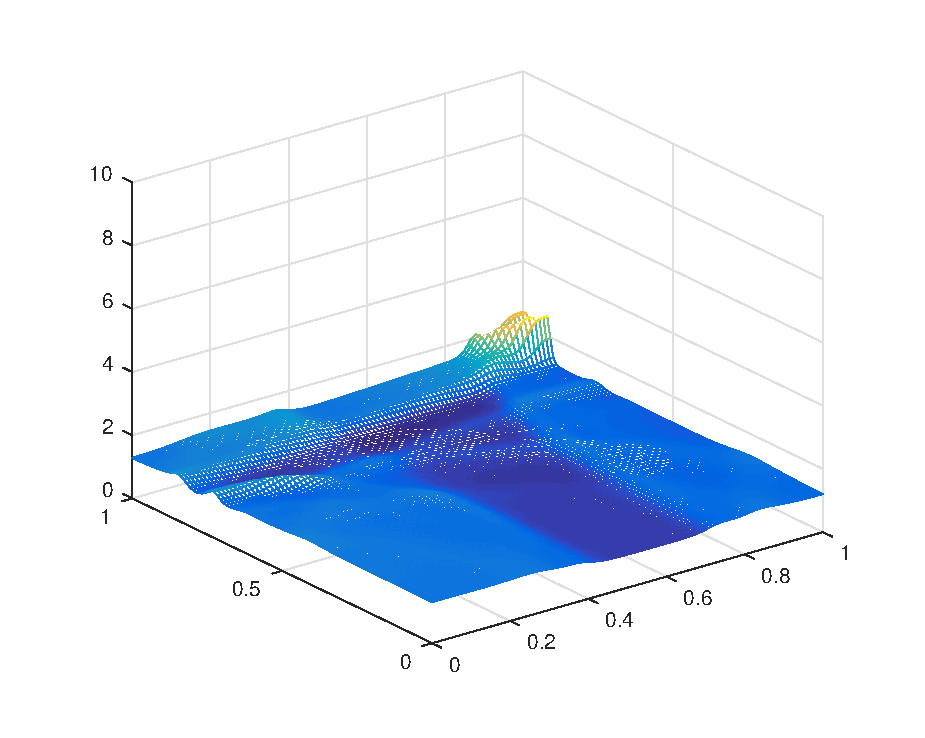
\includegraphics[width=\textwidth]{images/sol_ri_0800cf.eps}
        \caption{$n=800$}
        \label{fig:100}
    \end{subfigure}
    \begin{subfigure}[t]{0.48\textwidth}
        \centering
        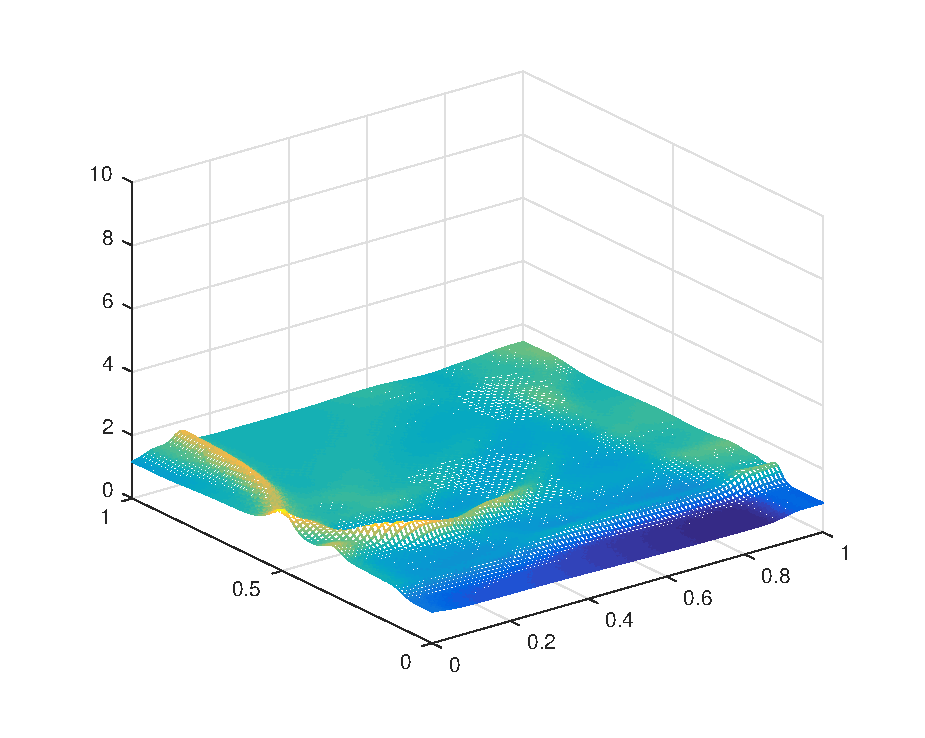
\includegraphics[width=\textwidth]{images/sol_ri_1000cf.eps}
        \caption{$n=1000$}
        \label{fig:100}
    \end{subfigure}
    \begin{subfigure}[t]{0.48\textwidth}
        \centering
        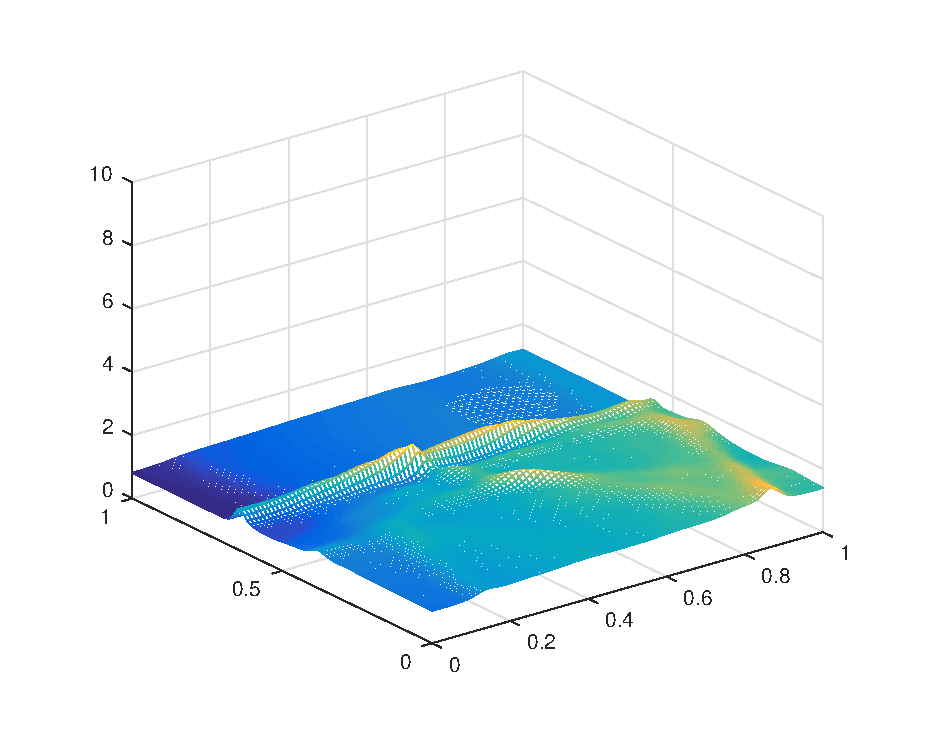
\includegraphics[width=\textwidth]{images/sol_ri_1200cf.eps}
        \caption{$n=1200$}
        \label{fig:999}
    \end{subfigure}
     \begin{subfigure}[t]{0.48\textwidth}
        \centering
        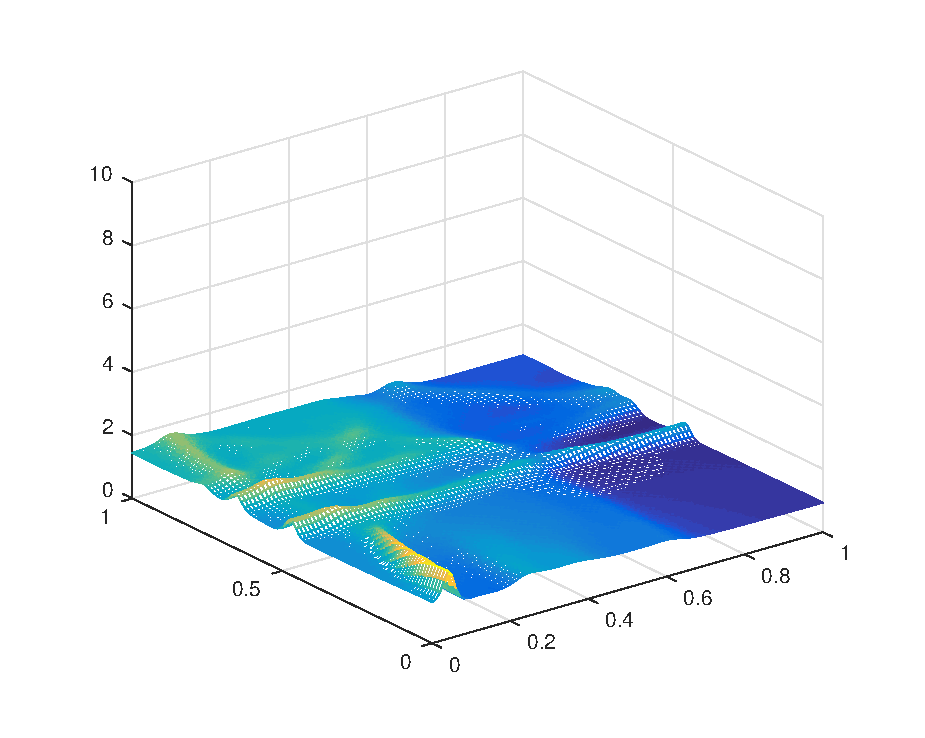
\includegraphics[width=\textwidth]{images/sol_ri_1400cf.eps}
        \caption{$n=1400$}
        \label{fig:999}
    \end{subfigure}
    \caption{Free boundary condtions for Richtmeyer scheme with Corilis force term.}
    \label{fig:2DSolutions_ri_cf}
\end{figure}





